\documentclass[a4paper, 12pt]{article}

% Adicionar pacotes:
\usepackage[top=2cm, bottom=2cm, left=1cm, right=1.5cm]{geometry} %Margens
\usepackage[utf8]{inputenc} %Acentuação
\usepackage{multirow} %Pacote usado para elaboração de tabelas
\usepackage{graphicx} %Pacote usado para adicionar imagens
\usepackage{tikz} %Pacote usado para desenhar os gráficos
\usepackage{amsmath} %Pacote de linguagem matemática

\begin{document}
	\begin{tabular}{|l|l|l|l|l|} \hline %Iniciar a tabela com 5 colunas e colocar a linha horizontal do topo da tabela
		\multirow{3}*{\includegraphics[width=35px]{LogoUFT.png}} & \multicolumn{4}{|l|}{\textbf{Universidade Federal do Tocantins - UFT}}\\ \cline{2-5} %Transformar a primeira coluna da tabela em uma só linha para preenche-la com a imagem
		& Professor: & \hspace{4cm} & Disciplina: & \hspace{4cm} \\ \cline{2-5} %Espaço de 4cm para coleta de dados
		& Estudante: & \hspace{6cm} & Matrícula: & \hspace{2cm}\\ \hline
	\end{tabular} %Final da tabela
	\bigskip
	
	\begin{center} %Centralizar a escrita
		Lista de exercícios \textbf{(exemplo)}
	\end{center} %Fim do texto que será centralizado

	\vspace{1.5cm}

	\begin{enumerate} %Início da contagem de itens da lista
		\item Primeiro texto. Assuma que existam apenas dois bens e suponha que o preço do bem 2 aumentou. Represente graficamente essa mudança. Se sabemos que o consumidor exaure toda a sua renda e prefere consumir mais a menos, esse aumento do preço do bem 2 irá afetar o seu bem-estar de que forma? Isso ocorrerá sempre? \\ %Enunciado da questão
		
			\begin{center} %Centralização do gráfico a ser desenhado
				\begin{tikzpicture}[scale=1] %Início do desenho e definição da escala
						%Eixos
					\draw[->, very thick] (-0.5,0) -- (8.8,0) node[right]{$x_1$}; %Eixo X1
					\draw[->, very thick] (0,-0.5) -- (0,8.8) node[above]{$x_2$}; %Eixo X2
						%Retas
					\draw (0,8) -- (8,0) node[below]{$\dfrac{m}{b}$}; %Primeira reta
					\draw (0,8) -- (5,0) node[below]{$\dfrac{m}{b'}$}; %Segunda reta
						%Complementos do gráfico
					\draw[->, very thick, red] (6.5,1) -- (5,1); %Seta que indica o sentido do movimento da reta
					\node[left] at (0,8){$\dfrac{m}{a}$}; %Dar nome para a intersecção com o eixo X2
				\end{tikzpicture} %Final do gráfico
			\end{center} %Final do ambiente centralizado

			\paragraph{} Supondo que há dois bens $a$ e $b$, temos uma representação normal do consumo destes dois bens quando o preço do bem $b$ aumenta, logo tem-se que o agente irá consumir menos, pois a sua renda $m$ é limitada. Dessa forma ocorre uma rotação na reta de consumo a partir do ponto de intersecção com o eixo que representa as quantidades consumidas do bem $a$, que permanece com seu consumo estático. Ou seja, esse aumento de preços gera perda de bem-estar, pois a utilidade total oferecida pelo consumo de $b$ irá diminuir, uma vez que é menos consumido e essa perda de utilidade não é compensada com outro bem. %Resposta da questão, com o uso do parágrafo

			\pagebreak %Quebra de página
		
		\item Curvas de indiferença. \\
			\begin{center} %Centralização do gráfico a ser desenhado
				\begin{tikzpicture}[scale=1] %Início do desenho e definição da escala
						%Eixos
					\draw[->, very thick] (0,0) -- (6.5,0) node[right]{Bem 1}; %Eixo do Bem 1
					\draw[->, very thick] (0,0) -- (0,6.5) node[above]{Bem 2}; %Eixo do Bem 2
						%Curvas
					\draw (1,6) to [out=280,in=175] (6,1) node[right]{$C_1$}; %Primeira curva
					\draw (2,6) to [out=280,in=175] (6,2) node[right]{$C_2$}; %Segunda curva
					\draw (3,6) to [out=280,in=175] (6,3) node[right]{$C_3$}; %Terceira curva
				\end{tikzpicture} %Final do gráfico
			\end{center} %Final da centralização

		\vspace{3cm}

		\item Oferta e demanda \\
			\begin{center} %Centralização do gráfico
				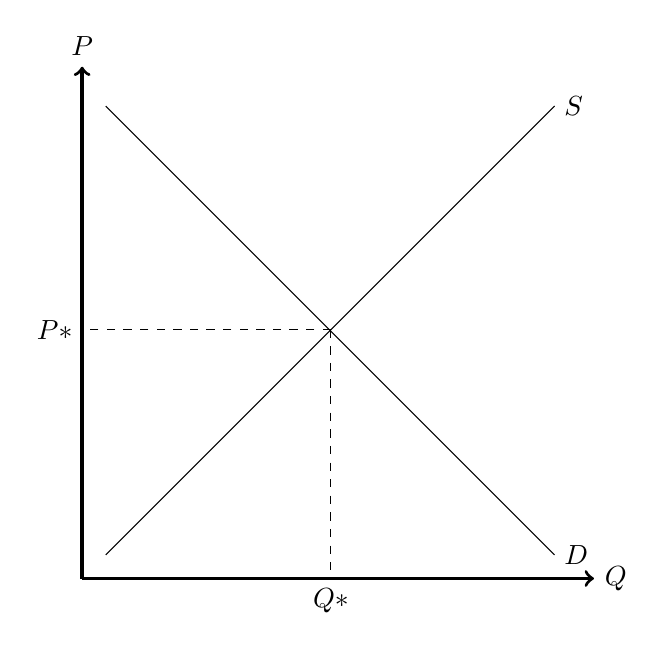
\begin{tikzpicture} %Início do gráfico
						%Eixos
					\draw[->, very thick] (0,0) -- (6.5,0) node[right]{$Q$}; %Eixo Q
					\draw[->, very thick] (0,0) -- (0,6.5) node[above]{$P$}; %Eixo P
						%Oferta e demanda
					\draw (0.3,0.3) -- (6,6) node[right]{$S$}; %Oferta
					\draw (0.3,6) -- (6,0.3) node[right]{$D$}; %Demanda
						%Equilíbrio
					\draw[dashed] (3.16,3.16) -- (3.16,0) node[below]{$Q*$}; %Linha tracejada que conecta o equilíbrio ao eixo Q
					\draw[dashed] (3.16,3.16) -- (0,3.16) node[left]{$P*$}; %Linha tracejada que conecta o equilíbrio ao eixo P
				\end{tikzpicture} %Finalização do gráfico
			\end{center}

			\pagebreak %Quebra de página		

		\item Função $y=x^2$ \\
				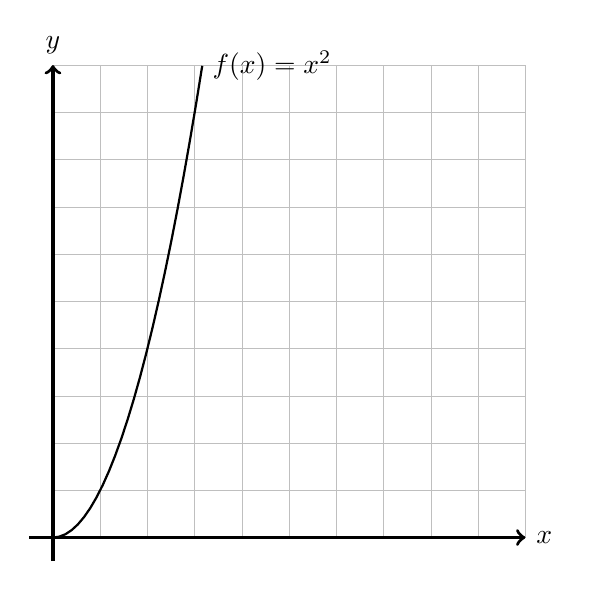
\begin{tikzpicture}[scale=0.6, domain=0:3.16] %Início do gráfico e definição da escala
					\draw[very thin,color=lightgray] (0,0) grid (10,10); %Contrução da grade
						%Eixos
					\draw[->, very thick] (-0.5,0) -- (10,0) node[right] {$x$}; %Eixo X
					\draw[->, very thick] (0,-0.5) -- (0,10) node[above] {$y$}; %Eixo Y
						%Plotagem da função
					\draw[thick] plot (\x,\x*\x) node[right] {$f(x)=x^2$}; %Função y=x^2
				\end{tikzpicture} %Finalização do gráfico

		\vspace{3cm}

		\item Função $y=2x$ \\
				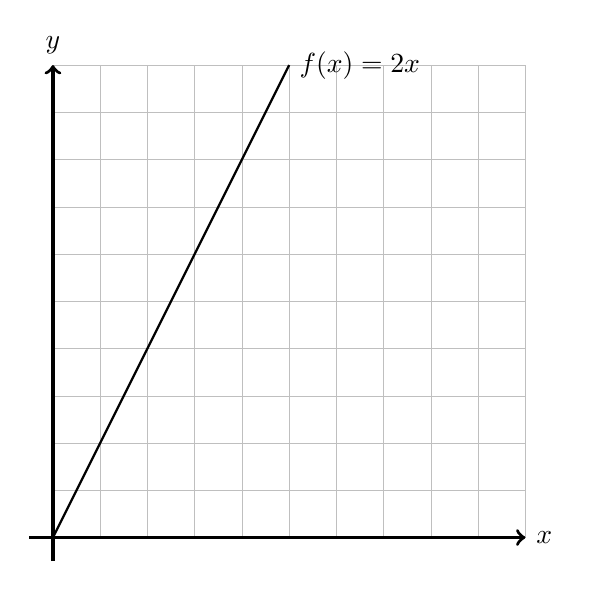
\begin{tikzpicture}[scale=0.6] %Início do gráfico
					\draw[very thin,color=lightgray] (0,0) grid (10,10); %Grade
						%Eixos
					\draw[->, very thick] (-0.5,0) -- (10,0) node[right] {$x$}; %Eixo X
					\draw[->, very thick] (0,-0.5) -- (0,10) node[above] {$y$}; %Eixo Y
						%Plotagem da função
					\draw[thick, domain=0:5] plot (\x,2*\x) node[right]{$f(x)=2x$}; %Função desejada 
				\end{tikzpicture} %Finalização do gráfico

		\pagebreak

		\item Plotagem de funções \\
			\begin{center}
				\begin{tikzpicture}[scale=0.6, domain=-10:10] %Início do gráfico e definição da escala e domínio
						%Eixos
					\draw[->, very thick] (-10.5,0) -- (10.5,0) node[right]{$x$}; %Eixo X
					\draw[->, very thick] (0,-10.5) -- (0,10.5) node[above]{$y$}; %Eixo Y
						%Plotagem de funções
					\draw[domain=-2.75:2.75, orange, thick] plot (\x,\x*\x+2) node[above]{$g(x)$}; %Função quadrática g(x)
					\draw[domain=-5:3, blue, thick] plot (\x,\x*2); %Primeira parte do sistema da equação f(x)
					\draw[domain=3:7, blue, thick] plot (\x,\x*-2+12) node[right]{$f(x)$}; %Segunda parte do sistema
					\draw[thick, brown] (-8,-6) -- (-1.5,-6); %Primeira parte do sistema da equação t(x)
					\draw[thick, brown] (-1.5,-6) to [out=5,in=265] (7,7) node[above]{$t(x)$}; %Segunda parte do sistema da equação t(x)
				\end{tikzpicture}
			\end{center}
	\end{enumerate}
\end{document}